\documentclass[9pt, xcolor=table]{beamer}

\usepackage[utf8]{inputenc}
\usepackage[round, comma]{natbib}
\usepackage{amsmath}
\usepackage{hyperref}
\usepackage{amsfonts}
\usepackage{verbatim}
\usepackage{makecell}
\usepackage{tikz}
\usetikzlibrary{shapes,arrows,positioning}
\usepackage{bbold}

\usepackage[round, comma]{natbib}

\DeclareMathOperator*{\argmin}{arg\,min}
\title[Interpretation of black box models]{Interpretation of black box models using tree-based surrogate models 
\newline \small{- Disputation -}} 
\author{Sofia Loibl}
\date{March 31\textsuperscript{th}, 2023}

\newcommand{\myname}{Sofia Maria Loibl}
\newcommand{\mysupervisor}{Dr. Giuseppe Casalicchio}


\mode<presentation> {

\usetheme{Madrid}

\setbeamertemplate{navigation symbols}{} 
\useinnertheme{circles}
\definecolor{greenish}{RGB}{0, 153, 76}
\usecolortheme[named=greenish]{structure}
}

\setbeamertemplate{headline}
{%
  \begin{beamercolorbox}[ht=3.5ex,dp=1.125ex,%
      leftskip=.3cm,rightskip=.3cm plus1fil]{section in head/foot}
    \usebeamerfont{section in head/foot}\usebeamercolor[fg]{section in head/foot}%
\insertsectionnavigationhorizontal{\paperwidth}{\hskip0pt plus1fill}{\hskip0pt plus1fill}
  \end{beamercolorbox}%
  \begin{beamercolorbox}[colsep=1.5pt]{middle separation line head}
  \end{beamercolorbox}
  \begin{beamercolorbox}[colsep=1.5pt]{lower separation line head}
  \end{beamercolorbox}
}
\setbeamerfont{itemize/enumerate subbody}{size=\normalsize} %to set the body size

\tikzstyle{block} = [rectangle, draw, fill=blue!20, text width=7em, text centered, rounded corners, minimum height=3em, font=\footnotesize]
\tikzstyle{line} = [draw, -latex']
\tikzstyle{cloud} = [draw, ellipse, node distance=3cm, text width=4em, text centered, minimum height=2em, font=\footnotesize]

      
\begin{document}

\begin{frame}
\begin{titlepage}
\begin{center}  

Department of Statistics \\
Ludwig-Maximilians-Universität München

\vspace{0.5cm}

\includegraphics[width = 0.15\textwidth]{sigillum.png}

\vspace{0.3cm}
\small
Supervised by Dr. Giuseppe Casalicchio

\end{center}
\end{titlepage}
\end{frame}


\begin{frame}
\frametitle{Table of contents} 
\tableofcontents 
\end{frame}

\section{Introduction}

\begin{frame}{Surrogate models}


\centering
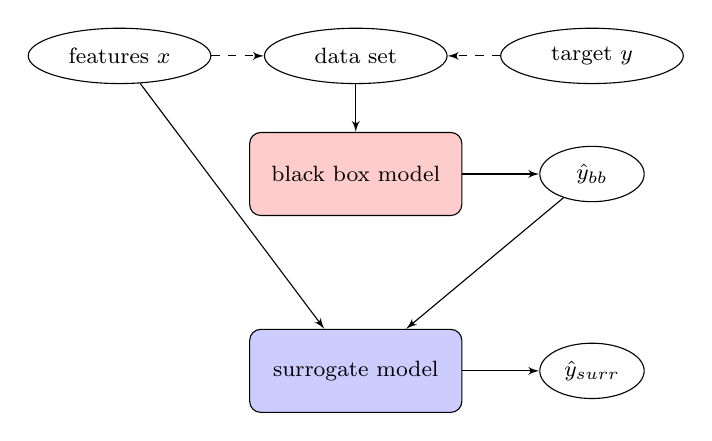
\begin{tikzpicture}[node distance = 2cm, auto]
    % Place nodes
    \node [cloud] (data) {data set};
    \node [cloud, left of=data] (features) {features $x$};
    \node [cloud, right of=data] (target) {target $y$};
    \node [block, below of=data, node distance=1.5cm, fill=red!20] (bb) {black box model};
    \node [cloud, below of=target, node distance=1.5cm, text width=2em] (bbpred) {$\hat{y}_{bb}$};
    \node [block, below of=bb, node distance=2.5cm] (surrogate) {surrogate model};
    \node [cloud, right of=surrogate, text width=2em] (surrpred) {$\hat{y}_{surr}$};
    % Draw edges
    \path [line] (data) -- (bb);
    \path [line,dashed] (features) -- (data);
    \path [line,dashed] (target) -- (data);
    \path [line] (bb) -- (bbpred);
    \path [line] (features) -- (surrogate);
    \path [line] (bbpred) -- (surrogate);
    \path [line] (surrogate) -- (surrpred);

\end{tikzpicture}
    
\end{frame}

\begin{frame}
 \centering
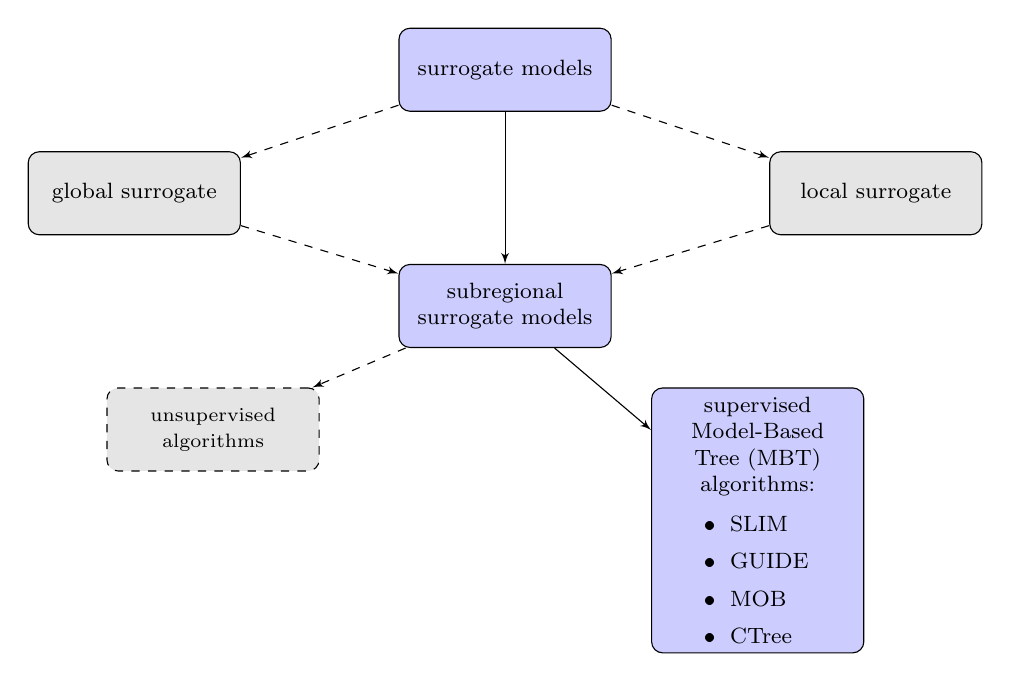
\begin{tikzpicture}[node distance = 2cm, auto]
    % Place nodes  
    \node [block] (surrogate) {surrogate models};
    \node [block, below left=0.5cm and 2cm of surrogate, fill=gray!20] (global) {global surrogate};
    \node [block, below right=0.5cm and 2cm of surrogate, fill=gray!20] (local) {local surrogate };
    \node [block, below of=surrogate, node distance=3cm] (subregional) {subregional surrogate models};
    \node[block, below left=0.5cm and 1cm of subregional, node distance=2cm, fill=gray!20, dashed, ] (unsupervised) {\scriptsize unsupervised algorithms};
    \node[block, below right=0.5cm and 0.5cm of subregional, node distance=2cm] (MBT) {supervised \\ Model-Based Tree (MBT) algorithms:\\
    \begin{itemize}
        \item SLIM
        \item GUIDE
        \item MOB
        \item CTree
    \end{itemize}};
   
    \path [line] (surrogate) -- (subregional);
    \path [line,dashed] (surrogate) -- (global);
    \path [line,dashed] (surrogate) -- (local);
    \path [line,dashed] (global) -- (subregional);
    \path [line,dashed] (local) -- (subregional);
    \path [line,dashed] (subregional) -- (unsupervised);
    \path [line] (subregional) -- (MBT);
    % Draw edges

\end{tikzpicture}   
\end{frame}




\begin{frame}{Goals}
\begin{itemize}
    \item  Comparison of four different algorithms for the generation of MBTs with regard to:
    \begin{itemize}
        \item Selection bias
        \item Performance 
        \item Interpretability
        \item Stability
    \end{itemize}
    \item Comparison of interpretability and performance for different model classes fitted in the subregions
    \item Investigate the suitability of MBTs as surrogate model
\end{itemize}

\end{frame}


\section{Model-based trees}
\begin{frame}
\centering
\huge{\textbf{Model-based trees}}
\begin{figure}
    \centering    
    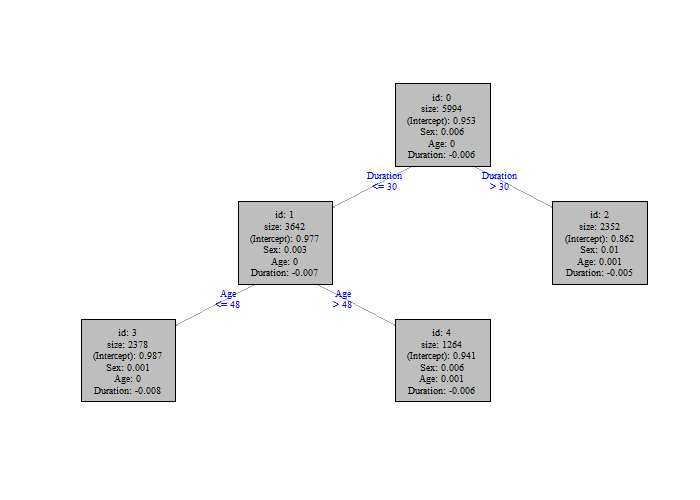
\includegraphics[width=12cm]{Figures/disputation/slim_lm_tree.png}
\end{figure}
\end{frame}

\begin{frame}{Requirements}

\textbf{Requirements for MBTs in this thesis}:
\begin{itemize}
    \item split by interactions
    \item main effect models in the subregions (nodes)
    \item flexible choice of main effect models (i.e. different objectives, regularized Regression, GAMs, ...)
    \item use features as potential splitting and regressor variables
\end{itemize}  
\end{frame}


\begin{frame}{Comparison of the algorithms}
\begin{table}[ht]
\centering \footnotesize
\begin{tabular}{|l|cccc|}
\hline
 & SLIM & MOB & CTree & GUIDE \\
\hline
\makecell[l]{Split point \\ selection} & exhaustive search & two-step & two-step & two-step \\
\hline
Test & - & \makecell[c]{score-based  \\ M-fluctuation test} & \makecell[c]{score-based  \\ permutation test} & \makecell{residual-based \\ $\chi^2$ test} \\
\hline
Flexibility & high & low & low & high \\
\hline
\makecell[l]{Distinction between \\ regressor and \\ splitting variables} & no & partly & partly & partly \\
\hline
Prepruning & improvement & alpha & alpha & improvement\\
\hline
Implementation & - & R package & R package & binary executable \\
\hline
\end{tabular}
\caption{Comparison of MBT algorithms - Methodology}
\label{tab:mbt_comparison}
\end{table}
    
\end{frame}



    

\section{Selection bias}
\begin{frame}
\centering
    \huge{\textbf{Selection bias}}
\end{frame}

\begin{frame}{Selection bias - Independence}
\textbf{Definition unbiased for an independent target:} \\
According to \citep{Hothorn.2006} an algorithm for recursive partitioning is called unbiased when, under the conditions of the null hypothesis of independence between a response $y$ and feature $\textbf{x}_{1},...\textbf{x}_{p}$ the probability of selecting feature $\textbf{x}_{j}$ is $1/p$ for all $j = 1,...,p$ regardless of the measurement scales or number of missing values. 

\vspace{0.5cm}
\textbf{Problem:} if an algorithm is biased in the case of independence, there is also a higher risk or bias if main effects of interactions are present
    
\end{frame}

\begin{frame}{Simulation independence}

\begin{table}[ht]
\centering 
\begin{tabular}{|l|cccc|}
\hline
 & SLIM & MOB & CTree & GUIDE \\
\hline
Designation & biased & \multicolumn{3}{|c|}{so called "unbiased"} \\
  \hline
\makecell[l]{simulation numerical - numerical} & biased & unbiased & unbiased & unbiased \\
\makecell[l]{simulation numerical - binary} & biased & unbiased & unbiased & unbiased \\
\makecell[l]{simulation numerical - categorical} & biased & biased & biased & biased \\
\hline
\end{tabular}
\caption{Comparison of MBT algorithms - Selection bias independence}
\end{table}
    
\end{frame}


\begin{frame}{Simulation interactions \\
- selection bias vs. splitting strategy}

\onslide<1,2>{
\begin{table}[!htb]
    \centering \footnotesize
    \begin{tabular}{lcll}
        \hline
        scenario & $\textbf{x}_1$,  $\textbf{x}_2$, $\textbf{x}_4$  & $\textbf{x}_3$ & $f(\textbf{x})$\\
        \hline
        numerical vs numerical & $[0,1]$ & \textcolor{teal}{$\{0, 0.1,..., 0.9, 1\}$}  &  $\mathbb{1}_{(\textbf{x}_1 \leq  mean(\textbf{x}_1))}\textbf{x}_2  +  \textcolor{teal}{\mathbb{1}_{(\textbf{x}_3 \leq  mean(\textbf{x}_3))}}\textbf{x}_4 $ \\
        numerical vs binary & $[0,1]$ & \textcolor{teal}{$\{0,1\}$} & $\mathbb{1}_{(\textbf{x}_1 \leq  mean(\textbf{x}_1))}\textbf{x}_2  +  \textcolor{teal}{\mathbb{1}_{(\textbf{x}_3 = 0)}}\textbf{x}_4$ \\
        \hline
    \end{tabular}
    \caption{scenarios selection bias interaction}
    \label{tab:selection_bias_interaction}
\end{table}
}

\onslide<2>{
\begin{figure}[!htb]
    \centering   
    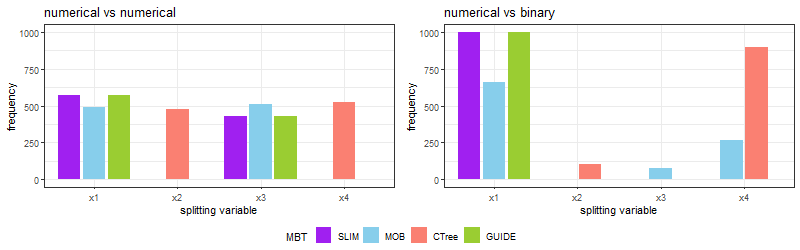
\includegraphics[width = 12cm]{Figures/disputation/interactions.png}
    \caption{Simulated frequencies of  first selected splitting features for the four interaction scenarios}
\end{figure}
}

\end{frame}

    

\section{Performance, Interpretability and Stability}
\begin{frame}
\centering
    \huge{\textbf{Comparison of performance, interpretability and stability}}
\end{frame}


\begin{frame}{Simulation - Comparison of Algorithms}
How do the algorithms differ in terms of
\begin{itemize}
    \item performance: $R^2$
    \item interpretability: number of leafnodes
    \item stability: variability of number of leafnodes and Rand Index
    \end{itemize}
in different simulation scenarios?

\vspace{0.3cm }
Main difference between scenarios: smooth interactions vs. subgroup depending effects

\vspace{0.5cm }
Additional Variations:
\begin{itemize}
    \item include correlation between features
    \item add noisy features
\end{itemize}

\end{frame}

\begin{frame}{Main results}
    \begin{itemize}
    \item Superiority of SLIM and GUIDE regarding interpretability and performance in subgroup detection tasks
    \item MOB and CTree show higher stability and slightly higher performance in scenarios with smooth interactions than SLIM and GUIDE 
    \item Pruning with SLIM and GUIDE not optimal, as strongly asymmetrical trees are sometimes generated (scenario linear smooth)
    \item Stability tends to be higher when MBTs are used as surrogate models
    \item SLIM and GUIDE more frequently split by wrong variables when correlated or noisy features are added
    \item Fundamental problem: modelling of smooth interactions with high performance only possible through many binary splits \\
     $\Longrightarrow$ strong decrease in interpretability 
\end{itemize}
\end{frame}


\begin{frame}{Simulation - Comparison of SLIM MBTs with leaf node models of different complexity}
\textbf{Question:} How do SLIM trees with models of different complexity in the leafnodes differ in terms of interpretability if non-linearities are present in the data?




\begin{table}
    \centering
    \begin{tabular}{l|lll}
    \hline
    & linear regression & polynomial lasso regression & GAM \\
    \hline
    Number of leafnodes & high & medium & low \\
    \hline
    \makecell[l]{Interpretability \\ of parameter estimates} & yes & partly & no \\
    \hline
    \makecell[l]{Separation of \\ interactions and \\ maineffects} & no & medium & yes \\
    \hline
    
    \end{tabular}
    \caption{Interpretability results of SLIM MBTs with different models based on simulation; Prepruning by $R^2$}
\end{table}

\end{frame}



\section{Conclusion}
\begin{frame}{Conclusion}
\begin{itemize}
    \item SLIM and GUIDE are promising surrogate models, especially when subgroups are present \\
    $\Longrightarrow$ R-package
    \item Improve pruning for SLIM and GUIDE
    \item For very deep MBTs the results of different MBT algorithms move closer together
    \item Use models that can capture non-linearities
    \item Beware of the risk of selection bias
\end{itemize}
    
\end{frame}


\begin{frame}{Bibliography}
\bibliography{bibliography}
\bibliographystyle{dcu}
\end{frame}


\begin{frame}{Scenario linear categorical}
 Numerical and binary features with linear effects and subgroup specific linear effects:
\begin{itemize}
    \item $\textbf{x}_1, \textbf{x}_2 \sim U(-1,1)$, $\textbf{x}_3 \sim Bern(0.5)$,  
    \item $ f(x) =  \textbf{x}_{1} - 8  \textbf{x}_2 + 16  \textbf{x}_2  \mathbb{1}_{(\textbf{x}_3 = 0)} + 8  \textbf{x}_2  \mathbb{1}_{(\textbf{x}_1 > mean(\textbf{x}_1))} $
    \item $\epsilon \sim N(0, 0.1 \cdot sd(f(\textbf{x}))$
    \item $y = f(\textbf{x}) + \epsilon$          
\end{itemize}   


\begin{table}
\centering \scriptsize
\begin{tabular}[t]{l|r|r|r|r|r|r|r}
\hline
MBT & $impr$ & n leaves & n leaves min & n leaves max & $R^2_{test}$ & sd $R^2_{test}$ & share $\textbf{x}_2$\\

\hline
SLIM & 0.15 & 2.00 & 2 & 2 & 0.8323 & 0.0118 & 0.0000\\
SLIM & 0.10 & 4.00 & 4 & 4 & 0.9870 & 0.0029 & 0.0000\\
SLIM & 0.05 & 4.00 & 4 & 4 & 0.9870 & 0.0029 & 0.0000\\
GUIDE & 0.15 & 2.00 & 2 & 2 & 0.8323 & 0.0118 & 0.0000\\
GUIDE & 0.10 & 4.00 & 4 & 4 & 0.9870 & 0.0029 & 0.0000\\
GUIDE & 0.05 & 4.00 & 4 & 4 & 0.9870 & 0.0029 & 0.0000\\
\hline
& $alpha$ & & & & & & \\
\hline
MOB & 0.001 & 13.45 & 11 & 16 & 0.9729 & 0.0069 & 0.8865\\
MOB & 0.010 & 14.38 & 13 & 16 & 0.9765 & 0.0066 & 0.8656\\
MOB & 0.050 & 14.63 & 13 & 16 & 0.9771 & 0.0062 & 0.8614\\
CTree & 0.001 & 11.96 & 10 & 14 & 0.9545 & 0.0049 & 0.9914\\
CTree & 0.010 & 12.76 & 10 & 15 & 0.9550 & 0.0050 & 0.9897\\
CTree & 0.050 & 13.46 & 10 & 16 & 0.9558 & 0.0052 & 0.9838\\
\hline
xgboost &  &  &  &  & 0.9778 & 0.9778 & \\
\hline
\end{tabular}
\caption{Mean simulation results on 100 simulation runs as surrogate models for XGBoost predictions; n = 1500}
\end{table}
\end{frame}

\end{document}